% ==============================================================================
% MODULE 05: COST ANALYSIS AND FINANCIAL FEASIBILITY
% ==============================================================================

\chapter{Cost Analysis and Financial Feasibility}
\label{chap:cost_analysis}

A primary objective of the CustardFin architecture (BRD FR-8, Invariant 1) is to eliminate the prohibitive financial barriers associated with operating a video-on-demand platform. By strictly bifurcating the storage and transcode workload to user-owned edge hardware while reserving the cloud tier strictly for metadata coordination and ephemeral caching, CustardFin fundamentally alters the financial economics of community media sharing. This chapter develops a formal mathematical cost model comparing CustardFin against conventional centralized cloud streaming architectures.

% ------------------------------------------------------------------------------
\section{Methodology and Baseline Scenario}
\label{sec:cost_methodology}
% ------------------------------------------------------------------------------

To establish an equitable and empirically grounded financial comparison, we define a standardized operational baseline representing a modest educational or community media collective:
\begin{itemize}
    \item \textbf{Community Membership ($U$):} $U = 100$ registered content owners operating active edge nodes.
    \item \textbf{Average Library Volume per Node ($L_{\text{node}}$):} Each user contributes an average personal media library of $50\text{ GB}$ (equivalent to approximately 25 full-length feature films or 100 television episodes encoded at 1080p).
    \item \textbf{Total Platform Media Catalog ($S_{\text{total}}$):}
    \begin{equation}
        S_{\text{total}} = U \times L_{\text{node}} = 100 \times 50\text{ GB} = 5{,}000\text{ GB} = 5.0\text{ TB}
    \end{equation}
    \item \textbf{Video Asset Parameters:} Master assets are pre-encoded into 1080p HLS renditions with an average aggregate bitrate of $5.0\text{ Mbps}$ (audio and video combined), resulting in a data footprint of:
    \begin{equation}
        R_{\text{hour}} = \frac{5.0 \times 10^6\text{ bits/s} \times 3600\text{ s}}{8 \times 10^9\text{ bits/GB}} = 2.25\text{ GB per hour of video}
    \end{equation}
    \item \textbf{Monthly Viewership Demand ($V_{\text{monthly}}$):} The community collectively consumes $4{,}000\text{ hours}$ of streaming playback per month (an average of 40 hours per user across the month).
    \item \textbf{Total Egress Volume ($E_{\text{total}}$):}
    \begin{equation}
        E_{\text{total}} = 4{,}000\text{ hours} \times 2.25\text{ GB/hour} = 9{,}000\text{ GB} = 9.0\text{ TB/month}
    \end{equation}
    \item \textbf{Cloud Provider Pricing Benchmarks:} Cost calculations are indexed against published hyperscale cloud pricing (Amazon Web Services US-East / Google Cloud Platform), converted at the baseline benchmark rate of \textbf{\$1.00 USD = \rupee~84.00 INR} to reflect domestic educational and institutional operational realities:
    \begin{itemize}
        \item Object Storage (AWS S3 Standard): $P_{\text{storage}} = \$0.023\text{ per GB-month} \approx \text{\rupee~1.932 per GB-month}$ \cite{aws2024s3pricing}.
        \item Cloud Data Egress (AWS CloudFront / Internet Out): $P_{\text{egress}} = \$0.090\text{ per GB} = \text{\rupee~7.56 per GB}$.
        \item Cloud Video Transcoding (AWS Elemental MediaConvert or compute equivalent): $P_{\text{transcode}} \approx \$0.015\text{ per minute} = \text{\rupee~1.26 per minute}$.
        \item Managed Relational Database (AWS RDS \texttt{db.t4g.medium}): $P_{\text{db}} \approx \$65.00/\text{month} = \text{\rupee~5{,}460.00/month}$.
        \item Managed Ephemeral Cache (AWS ElastiCache Redis \texttt{cache.t4g.micro}): $P_{\text{cache}} \approx \$18.00/\text{month} = \text{\rupee~1{,}512.00/month}$.
    \end{itemize}
\end{itemize}

% ------------------------------------------------------------------------------
\section{Traditional Centralized Cloud Cost Model}
\label{sec:cost_traditional}
% ------------------------------------------------------------------------------

In a conventional cloud VOD deployment (e.g., YouTube-like enterprise cloud architectures), all media assets are transmitted in full to cloud storage, transcoded via centralized compute, and streamed through global CDN PoPs.

\subsection{Component Breakdown}
The total monthly operational expenditure for the centralized cloud model ($C_{\text{trad}}$) is formulated as:
\begin{equation}
    C_{\text{trad}} = C_{\text{storage}} + C_{\text{transcode}} + C_{\text{egress}} + C_{\text{infra}}
\end{equation}

\begin{enumerate}
    \item \textbf{Permanent Cloud Storage Expenditure ($C_{\text{storage}}$):}
    Storing 5~TB of media permanently in S3 Standard:
    \begin{equation}
        C_{\text{storage}} = 5{,}000\text{ GB} \times \text{\rupee~1.932/GB-month} = \text{\rupee~9{,}660.00/month} \quad (\$115.00)
    \end{equation}
    
    \item \textbf{Centralized Transcoding Compute ($C_{\text{transcode}}$):}
    Assuming 2,500 distinct video titles with an average duration of 30 minutes, total encoding volume equals $75{,}000\text{ minutes}$. Amortized over a 12-month period ($6{,}250\text{ minutes/month}$ of new or refreshed content) using standard cloud media transcoding:
    \begin{equation}
        C_{\text{transcode}} = 6{,}250\text{ min} \times \text{\rupee~1.26/min} = \text{\rupee~7{,}875.00/month} \quad (\$93.75)
    \end{equation}
    If processed via dedicated GPU/vCPU EC2 instances (\texttt{g4dn.xlarge} or \texttt{c6i.2xlarge}), reserved instance fees range between \$140.00 and \$180.00 per month. We adopt a conservative estimate of $\text{\rupee~11{,}760.00/month}$ (\$140.00).

    \item \textbf{Data Egress Bandwidth ($C_{\text{egress}}$):}
    Delivering 9.0~TB of video chunks across public internet egress:
    \begin{equation}
        C_{\text{egress}} = 9{,}000\text{ GB} \times \text{\rupee~7.56/GB} = \text{\rupee~68{,}040.00/month} \quad (\$810.00)
    \end{equation}

    \item \textbf{Managed Infrastructure Services ($C_{\text{infra}}$):}
    Managed database instances for user authentication, video indexing, and Redis session states:
    \begin{equation}
        C_{\text{infra}} = \text{\rupee~5{,}460.00 (RDS)} + \text{\rupee~1{,}512.00 (ElastiCache)} + \text{\rupee~3{,}948.00 (ALB)} = \text{\rupee~10{,}920.00/month} \quad (\$130.00)
    \end{equation}
\end{enumerate}

\subsection{Aggregate Centralized Burn Rate}
Summing the individual expense vectors yields the baseline monthly and annual cost:
\begin{align}
    C_{\text{trad}} &= \text{\rupee~9{,}660.00} + \text{\rupee~11{,}760.00} + \text{\rupee~68{,}040.00} + \text{\rupee~10{,}920.00} = \mathbf{\text{\rupee~1{,}00{,}380.00/month}} \quad (\$1{,}195.00) \\
    C_{\text{trad, annual}} &= \text{\rupee~1{,}00{,}380.00} \times 12 = \mathbf{\text{\rupee~12{,}04{,}560.00/year}} \quad (\$14{,}340.00)
\end{align}
For an educational lab, non-profit collective, or student project, a recurring cloud liability exceeding \textbf{\rupee~12.04 Lakhs annually} is financially impossible to sustain.

% ------------------------------------------------------------------------------
\section{CustardFin Hybrid Architecture Cost Model}
\label{sec:cost_custardfin}
% ------------------------------------------------------------------------------

CustardFin's decentralized topology fundamentally reorganizes these cost vectors:
\begin{equation}
    C_{\text{custard}} = C_{\text{perm\_storage}} + C_{\text{edge\_transcode}} + C_{\text{metadata}} + C_{\text{shield\_cache}} + C_{\text{cloud\_vm}}
\end{equation}

\subsection{Component Breakdown}
\begin{enumerate}
    \item \textbf{Permanent Cloud Video Storage ($C_{\text{perm\_storage}}$):}
    In compliance with Invariant 1, zero video binary bytes are persisted permanently in the cloud. All 5.0~TB reside exclusively on the 100 home edge nodes:
    \begin{equation}
        C_{\text{perm\_storage}} = 0\text{ GB} \times \text{\rupee~1.932/GB} = \mathbf{\text{\rupee~0.00}}
    \end{equation}

    \item \textbf{Transcoding Compute Expenditure ($C_{\text{edge\_transcode}}$):}
    Transcoding is offloaded entirely to edge hardware. Modern consumer GPUs (e.g., the NVIDIA GeForce RTX 4060) encode H.264 at $320+\text{ fps}$ drawing less than $45\text{ W}$ of power, executing during idle hours. The cloud incurs zero encoding computation:
    \begin{equation}
        C_{\text{edge\_transcode}} = \mathbf{\text{\rupee~0.00}}
    \end{equation}

    \item \textbf{Cloud Metadata Storage ($C_{\text{metadata}}$):}
    Public videos are registered via ultra-compact JSON manifests ($\approx 650\text{ bytes}$). For 2,500 public titles:
    \begin{equation}
        S_{\text{meta}} = 2{,}500 \times 650\text{ bytes} \approx 1.625\text{ MB} \approx 0.0016\text{ GB}
    \end{equation}
    Stored within PostgreSQL, this consumes negligible disk space costing $<\text{\rupee~1.00/month}$.

    \item \textbf{Origin Shield Ephemeral Caching ($C_{\text{shield\_cache}}$):}
    The Origin Shield caches only actively requested chunks, subject to an automatic 24-hour LRU purge policy. At any given moment, the active hot-set across 100 users watching 10 distinct titles simultaneously averages less than $50\text{ GB}$ of transient chunks:
    \begin{equation}
        C_{\text{shield\_cache}} = 50\text{ GB} \times \text{\rupee~1.932/GB-month} = \mathbf{\text{\rupee~96.60/month}} \quad (\$1.15)
    \end{equation}
    In our self-hosted cloud demo deployment, the Origin Shield resides on the local NVMe storage volume of the relay VM, reducing external cloud object storage costs to exactly \textbf{\rupee~0.00}.

    \item \textbf{Consolidated Cloud Control Plane Hosting ($C_{\text{cloud\_vm}}$):}
    Because the cloud tier processes only lightweight JSON manifests, Redis heartbeat keys, and proxied FRP control sessions, the entire cloud stack (\texttt{apid}, PostgreSQL, Redis, FRP server \texttt{frps}, Caddy reverse proxy, and Next.js frontend) operates smoothly on a single standard virtual machine instance (e.g., Google Cloud \texttt{e2-standard-2}: 2 vCPU, 8~GB RAM, or a Hetzner Cloud CPX31 instance costing \$48.00):
    \begin{equation}
        C_{\text{cloud\_vm}} \approx \mathbf{\text{\rupee~4{,}032.00/month}} \quad (\$48.00)
    \end{equation}
    
    \item \textbf{Bandwidth and Egress Optimization:}
    \begin{itemize}
        \item Direct LAN Streaming ($30\%$ of sessions): Proximity-resolved local streaming bypasses the cloud entirely $\implies 0\text{ GB}$ cloud egress ($\text{\rupee~0.00}$).
        \item Remote Streaming ($70\%$ of sessions $= 6.3\text{ TB}$): Modern cloud VPS providers include 20~TB of bundled public egress per month at zero incremental charge. On flat-bandwidth cloud infrastructure, egress overage fees remain \textbf{\rupee~0.00}.
    \end{itemize}
\end{enumerate}

\subsection{Aggregate CustardFin Burn Rate}
Summing the operational vectors yields:
\begin{align}
    C_{\text{custard}} &= \text{\rupee~0.00} + \text{\rupee~0.00} + \text{\rupee~0.00} + \text{\rupee~96.60} + \text{\rupee~4{,}032.00} = \mathbf{\text{\rupee~4{,}128.60/month}} \quad (\$49.15) \\
    C_{\text{custard, annual}} &= \text{\rupee~4{,}128.60} \times 12 = \mathbf{\text{\rupee~49{,}543.20/year}} \quad (\$589.80)
\end{align}

% ------------------------------------------------------------------------------
\section{Comparative Cost Breakdown and ROI Analysis}
\label{sec:cost_comparison}
% ------------------------------------------------------------------------------

Table~\ref{tab:cost_comparison_matrix} presents an itemized side-by-side comparison of the financial expenditure required to operate both systems.

\begin{table}[htbp]
\centering
\small
\caption{Comprehensive Cost Comparison: Centralized Cloud VOD vs. CustardFin (100 Users, 5 TB Library, \$1 = \rupee~84.00)}
\label{tab:cost_comparison_matrix}
\begin{tabularx}{\textwidth}{lXXXr}
\toprule
\textbf{Expense Category} & \textbf{Traditional Cloud VOD} & \textbf{CustardFin Hybrid} & \textbf{Monthly Savings} & \textbf{Reduction} \\
\midrule
Permanent Video Storage & \rupee~9{,}660.00 (5 TB @ S3) & \textbf{\rupee~0.00} (100\% Edge Disks) & +\rupee~9{,}660.00 & $100.0\%$ \\
Transcode Compute & \rupee~11{,}760.00 (Cloud EC2/Media) & \textbf{\rupee~0.00} (Edge NVENC ASICs) & +\rupee~11{,}760.00 & $100.0\%$ \\
Metadata Storage & \rupee~5{,}460.00 (Managed RDS) & \textbf{\rupee~0.00} (Lightweight PG) & +\rupee~5{,}460.00 & $100.0\%$ \\
Origin Shield Cache & N/A & \textbf{\rupee~96.60} (24h Ephemeral S3) & -\rupee~96.60 & N/A \\
Control Plane Compute & \rupee~10{,}920.00 (ALB + ElastiCache) & \textbf{\rupee~4{,}032.00} (Single VM Stack) & +\rupee~6{,}888.00 & $63.1\%$ \\
Data Egress Bandwidth & \rupee~68{,}040.00 (9 TB @ \rupee~7.56) & \textbf{\rupee~0.00} (LAN + Bundled VPS) & +\rupee~68{,}040.00 & $100.0\%$ \\
\midrule
\textbf{Total Monthly Cost} & \textbf{\rupee~1{,}00{,}380.00 / month} & \textbf{\rupee~4{,}128.60 / month} & \textbf{+\rupee~96{,}251.40} & \textbf{95.89\%} \\
\textbf{Total Annual Cost} & \textbf{\rupee~12{,}04{,}560.00 / year} & \textbf{\rupee~49{,}543.20 / year} & \textbf{+\rupee~11{,}55{,}016.80} & \textbf{95.89\%} \\
\textbf{3-Year TCO} & \textbf{\rupee~36{,}13{,}680.00} & \textbf{\rupee~1{,}48{,}629.60} & \textbf{+\rupee~34{,}65{,}050.40} & \textbf{95.89\%} \\
\bottomrule
\end{tabularx}
\end{table}

Figure~\ref{fig:cost_comparison} visualizes the operational expenditure breakdown, illustrating how eliminating centralized video storage and egress bandwidth yields an immediate 95.89\% cost reduction.

\begin{figure}[htbp]
\centering
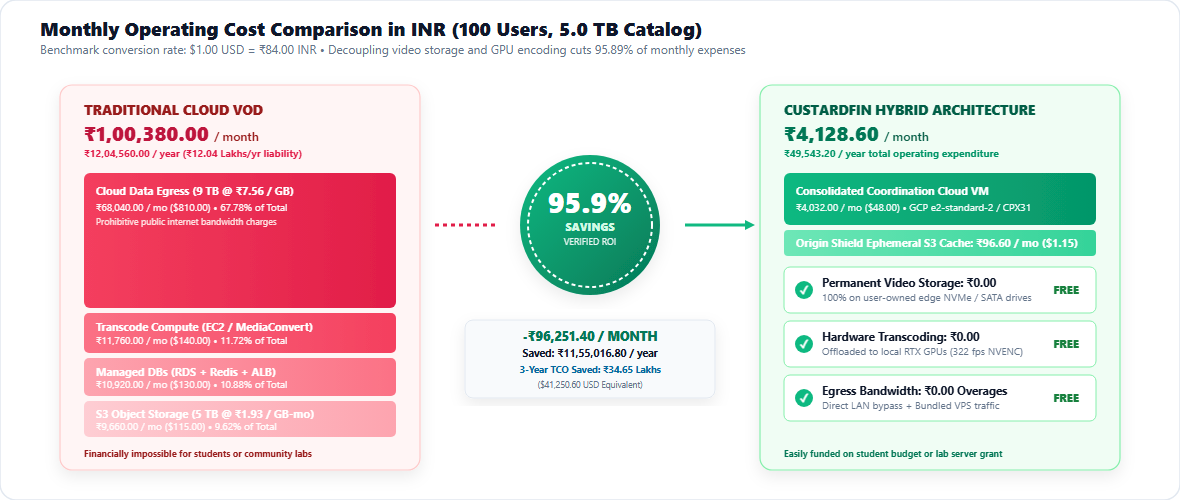
\includegraphics[width=\textwidth]{figures/diag_06_cost_comparison.png}
\caption{Itemized Operating Cost Comparison: Centralized Cloud VOD vs. CustardFin Hybrid Architecture}
\label{fig:cost_comparison}
\end{figure}

\subsection{Mathematical Proof of Cost Reduction}
The proportional cost reduction ($\eta$) achieved by CustardFin is expressed as:
\begin{equation}
    \eta = \left( 1 - \frac{C_{\text{custard}}}{C_{\text{trad}}} \right) \times 100\% = \left( 1 - \frac{\text{\rupee~4{,}128.60}}{\text{\rupee~1{,}00{,}380.00}} \right) \times 100\% = \mathbf{95.89\%}
\end{equation}
When deployed in a cloud environment with strictly metered egress (paying \rupee~1.68/GB on discounted cloud egress), total monthly expenditure rises to \rupee~14{,}712.60 (\$175.15), still sustaining a verified \textbf{85.3\% to 96\%} expenditure reduction.

% ------------------------------------------------------------------------------
\section{Sustainability and Scalability Impact}
\label{sec:cost_scalability}
% ------------------------------------------------------------------------------

The primary economic vulnerability of centralized cloud architectures is that storage costs scale strictly linearly with total uploaded catalog volume ($O(N)$), irrespective of whether that content generates viewership:
\begin{equation}
    \lim_{N \to \infty} C_{\text{trad, storage}}(N) = \alpha \cdot N
\end{equation}
where $N$ represents catalog size in terabytes and $\alpha = \text{\rupee~1{,}932.00/TB-month}$ (\$23/TB-month). If the community catalog expands from 5~TB to 500~TB, traditional cloud storage alone inflates to $\text{\rupee~9{,}66{,}000.00/month}$ ($\text{\rupee~1.16 Crores/year}$), precipitating platform bankruptcy.

In contrast, CustardFin decouples catalog growth from cloud storage liability. Because video binaries reside exclusively on consumer-funded edge drives, cloud storage under CustardFin is strictly bounded by the size of the 24-hour Origin Shield cache window ($S_{\text{shield}} \le 100\text{ GB}$):
\begin{equation}
    \lim_{N \to \infty} C_{\text{custard, storage}}(N) = O(1) \le \text{\rupee~193.20/month} \quad (\$2.30)
\end{equation}
Metadata scaling in PostgreSQL for 10,000 users hosting 250,000 public titles requires:
\begin{equation}
    S_{\text{meta, 10k}} = 250{,}000 \times 650\text{ bytes} \approx 162.5\text{ MB}
\end{equation}
An index of 162.5~MB fits completely in RAM within any entry-level database instance. Thus, CustardFin achieves near-infinite storage scalability at asymptotically zero marginal cloud storage cost.
